Para obtener las curvas características de fotocorriente, se montó una lámpara 
de mercurio en un extremo de una base metálica. A continuación, se colocó un 
diafragma regulable para ajustar la intensidad lumínica, seguido de un filtro 
de color azul o violeta. Finalmente, en el otro extremo de la base metálica, se
posicionó la fotocelda. Este montaje se muestra en la  
\cref{fig:experimental-setup}.

\begin{figure}[htbp!]
  \begin{center}
    \includegraphics[width=0.9\linewidth, page=2]{../Images/characteristics.pdf}
    \caption{Montaje experimental.}
    \label{fig:experimental-setup}
  \end{center}
\end{figure}

Para la toma de datos, se utilizó un picoamperímetro para medir la corriente y 
una resistencia variable para ajustar el voltaje. Para un filtro del mismo 
color, se variaron tres configuraciones de apertura del diafragma: 
completamente abierto, a una apertura media y lo más cerrado posible. 
La fuente de voltaje se fijó inicialmente en 5.1 V, y con la resistencia 
variable se tomaron cinco valores distintos de voltaje dentro de este rango. 
Luego, se midieron los valores de corriente correspondientes a esos voltajes.

Posteriormente, se invirtió la polaridad de la fuente de voltaje y se repitió 
el mismo procedimiento. Este proceso se realizó para las tres intensidades 
lumínicas antes de cambiar al segundo filtro y repetir la toma de datos.
